% Estilo general del documento:
	% Tamaño general:
	
	\documentclass[10pt]{beamer}
\setbeamertemplate{footline}[page number]
	\mode<presentation>{
		\usetheme{Hannover}				% Tema de la presentación.
		\usecolortheme[rgb={0.1, 0.5, 0.1}]{structure} 	% Color principal.
		\setbeamercovered{transparent} 			% Con este comando los ítems ocultos se muestran semitransparentes.
		\useinnertheme{rounded}


	}

\usepackage{pgf}
	% Mostrar el índice de nuevo al cambiar de sección:
	
	\AtBeginSection{
		\begin{frame}<beamer>{\'{I}ndice}
			\tableofcontents[currentsection,subsections]
		\end{frame}
	}
% Paquetes incluidos por defecto:
	% Tipo de fuente:
	
	\usepackage{palatino}

	% Justificación del texto:
	
	\renewcommand{\raggedright}{\leftskip=0pt \rightskip=0pt plus 0cm} 
	
	% Inclusión de imágenes:
	
	\usepackage{graphicx}
	\usepackage{epstopdf}
	
	% Matemáticos:

	\usepackage{amsmath, amssymb, latexsym}
	
	% De idioma:
	
	\usepackage[english,spanish]{babel}
	\usepackage[utf8x]{inputenc}
	\usepackage[T1]{fontenc}
	

\title{Practice Project}
\author{Jacinto Arias, Adrián Sánchez}
\institute{AI in Videogames \and University of Castilla-La Mancha}
\date{\today}

\logo{\includegraphics{loguete.png}}

\begin{document}

	\begin{frame}
		\titlepage
	\end{frame}

	\begin{frame}[plain]{}
	%  \begin{center}
	  \includegraphics[scale=0.2]{zlogo.png}
	 % \end{center}
	\end{frame}

	\begin{frame}{About Zproject}
	   \textbf{Zproject} is a game about zombies...
	    \newline

	   ...but this time you wouldn't want the zombies to be smashed.
	\end{frame}

	\begin{frame}{The zombies...}

	   \vspace{1cm}
	   You would control a horde of them. But they won't always obey you, because they need \textbf{food} (more brains).
	   \newline
	    
	   If the zombies are \textbf{hungry} they would do their own will!

	  \begin{center}
	  \includegraphics[scale=0.7]{zombies.png}
	  \end{center}
	\end{frame}


	\begin{frame}{The enemies...}

	   \vspace{1cm}
	   There are a few kind of enemies, such as Defensive Turrets, Flyers and Robots.
	   \newline
	    
	   Be careful because, if they can, will shoot you.
	  \begin{center}
	  \includegraphics[scale=0.7]{enemies.png}
	  \end{center}
	\end{frame}

	\begin{frame}{Your goal is...}

	   \vspace{1cm}
	   To get as many zombies you can to the enemy fortress.
	   \newline
	    
	   It's up to you to sacrifice the zombies or avoid the enemies. But we assure you it would be bloody...
	  \begin{center}
	  \includegraphics[scale=0.4]{goal.png}
	  \end{center}
	\end{frame}

	\begin{frame}{AI in videogames}
		\Large Let's talk about AI in videogames!
	\end{frame}

	\begin{frame}{Index}
		\tableofcontents
	\end{frame}

	\section{Videogame analysis}

  
	\begin{frame}{Classification}
	  \footnotesize
	  \begin{itemize}
	  \item \textbf{Game type:} Real Time Strategy.
	  \item \textbf{Type of use:} Machine controlling physics, ground generation and opponent.
	  \item \textbf{Theme:} Horde of units.
	  \item \textbf{User age:} Violence and horror, so +18.
	  \item \textbf{Skills development:} Spacial abilities and reasoning.
	  \item \textbf{Platform:} PC, \textit{Microsoft Windows} and \textit{Linux}.
	  \item \textbf{Technology development:} Ogre 3D, Blender, Gimp, OIS and OpenAl.
	  \item \textbf{Development company:} Jacinto \&\& Adrián || Adrián \&\& Jacinto Dev.
	  \item \textbf{Year of development:} 2012.
	  \end{itemize}
	\end{frame}

	\section{AI principles I: Computational Theory}

	  \subsection{Knowledge Extraction}

	  	\begin{frame}{Knowledge Extraction}
		  \begin{itemize}
		   \item Everything has to be accomplished by using a \textbf{large number} of units.
		    
		   \item You will control a few \textbf{groups}, make an strategy before giving orders to them.

		   \item You should \textbf{take a look} of the map before start to send all your units to an early end.

		   \item \textbf{Coordinate} your units to attack at once and corner the stronger enemies.

		   \item Avoid fighting far away enemies or turrets if you can. \textbf{Better skip} them.
		  \end{itemize}
		  
	  	\end{frame}

	  	\begin{frame}{In deep...}
		  Each unit in the game has stats, some enemies would be stronger and others faster.
		  \newline


		  \begin{itemize}
		   \item \textbf{Life:} Amount of damage that an unit can be dealt before die.
		   \item \textbf{Damage Per Second:} Amount of damage that an unit deal.
		   \item \textbf{Range:} Maximum distance that a unit can attack.
		   \item \textbf{Speed:} Velocity of the enemy displacements around the map.
		  \end{itemize}
	      \end{frame}

	    \subsection{Artificial intelligence applications}

		\begin{frame}{Movement problems}

		  Several movement problems have to be solved:
		\newline
		  \begin{itemize}
		   \item \textbf{Zombies} movement by direct input from the player.\newline
		   \item \textbf{Zombies} movement when acting by themselves: If the hunger level is low, we should apply a movement pattern based on some technique.\newline
		   \item \textbf{Enemies} movement: They are our opponent, so they must try to make the player loose. For this we could apply a random pattern or a AI system.\newline
		  \end{itemize}

		\end{frame}

	      \begin{frame}{Path finding and collision avoidance}
	       
		      We should include techniques in order to make both the zombies and enemies \textbf{not to pass through solid terrain} elements.
	  
		  \vspace{1cm}
		      Also a \textbf{collision system} must be included in order to make the units fight each others. Trace shoots or melee attacks.
	      \end{frame}


	      \begin{frame}{Opponent strategy}
		  \footnotesize

		  The problems to solve in order to make a good opponent are:

		    \begin{itemize}
		    \item Moving and positioning the units.
		    \item Look for, select and attack zombies.
		    \newline
		    \end{itemize}


		  We provide a framework to implement opponents AI:

		      \begin{itemize}
		      \item \textbf{Enemy behaviour:} There are two behaviours in which the enemy can be at a given moment:
			  \begin{itemize}  \footnotesize
			      \item \textit{Patrol}: The enemy is moving around the map.
			      \item \textit{Seek}: The enemy is rotating to searching zombies in range.
			    \end{itemize}

		      \item \textbf{Enemy aggressiveness:} The enemy can be in an aggressive mood or not. If aggressiveness is on, the enemy would shoot at anything that comes into range.
		      \item \textbf{Environment data:} The enemy can know at any moment about its own data and the zombies data over the map with no restriction.
		      \end{itemize}
	       
	      \end{frame}


	\section{AI principles II: Representation and algorithms}

	    \subsection{Application of search techniques}
    
	     
	      \begin{frame}{Path finding}
	      \small
	           \begin{itemize}
		    \item \textbf{Input space:}
		      \begin{itemize}
			 \footnotesize
			 \item The map divided in regions and represented as a non directed graph.
			 \item Each node will be either a passable or an impassable region.
			 \item Actual and desired final location.
		      \end{itemize}
		    \item \textbf{Output space:} The algorithm will return a valid path of the graph.
		    \item \textbf{States:} Each node of the graph. Only the nodes that are passable can be considered as valid states. 
		    \item \textbf{Initial-final state:} The initial location and the desired one.
		    \item \textbf{Operators:} Ramification through states should be done by moving directly to the neighbours of the current node.
		    \item \textbf{Function of heuristic evaluation:} The cost of going from the origin to the destination without considering the condition of the regions.
		   \end{itemize}
	      \end{frame}


	    \subsection{Application of rule based systems}

	    \begin{frame}{Simulation of a birds flock}
	    \small
	      \begin{itemize}
	      \item \textbf{Input space:} The unit location, and the other units location.
	      \item \textbf{Output space:} Destination where the unit will go.
	      \item \textbf{Input and output representation:} 2D points in a cartesian system.
	      \item \textbf{Statements base:} Nearest unit distance.
	      \item \textbf{Considerations for the inference engine:} The inference engine will be emulated using sequential conditionals.
	      \item \textbf{Set of rules (knowledge injected):} Ordered by highest priority:\newline
		  \begin{itemize}
		    \footnotesize
		    \item \textit{If you are far away from other birds, head toward the nearest bird.}
		    \item \textit{If you are about to crash into another bird, turn around.}
		    \item \textit{Otherwise, fly in the same direction as the bird next to you.}\newline
		  \end{itemize}
	      
	      \end{itemize}
	    \begin{center} 
	    \texttt{<Play demo \#001>}	     
	    \end{center}

	    \end{frame}


	    \begin{frame}{AI behaviour: The hunter}
	    \small
	     \begin{itemize}
	      \item \textbf{Input space:} Actual location, and the zombies locations.
	      \item \textbf{Output space:} Next action: move to, stay or seek for enemies.
	      \item \textbf{Input and output representation:} 2D points in a cartesian system.
	      \item \textbf{Statements base:} Previously attacked unit, nearest unit location.
	      \item \textbf{Considerations for the inference engine:} The inference engine will be emulated using sequential conditionals.
	      \item \textbf{Set of rules (knowledge injected):}\newline
		  \begin{itemize}
		    \footnotesize
		    \item \textit{If the nearer enemy is too close move away before attacking it.}
		    \item \textit{If an enemy gets in range, shoot at it.}
		    \item \textit{If you has just killed and enemy, stay and seek for the rest of the pack.}
		    \item \textit{If you don't have an objetive move closer to the nearer enemy.}
		  \end{itemize}

	      \end{itemize}
	    \begin{center} 
	    \texttt{<Play demo \#002>}	     
	    \end{center}

	    \end{frame}


	    \subsection{Other schemes}

	      \begin{frame}{Other schemes}
	       \footnotesize
		  \begin{itemize}
		   \item \textbf{CBR:}
		    \begin{itemize}
		    \footnotesize
		      \item Define some opponent strategies , giving more flexibility than a RBS.
		      \item The point of using CBR is that we can face it against human players to see how it \textbf{evolves}.
		      \item A good variation of this should be using it to adjust the selected strategies of each enemy in the map, like a \textbf{meta-algorithm}.\newline
		    \end{itemize}

		    \item \textbf{Conectionism:} The problem is the need of learning. The learning process is \textbf{more complex} and requires more simulations that would be really difficult to make without the intervention of an human player.\newline

		    \item \textbf{Evolutionary computation:} Can be used in order to optimize the game parameters like the units stats or generating levels in order to \textbf{automatically balance} the game.
		  \end{itemize}
	      \end{frame}

	    \subsection{Mathematical approaches and other algorithms}

	      \begin{frame}{Mathematical approaches and other algorithms used}
	       \begin{itemize}
		   \item \textbf{Collision system and geometry navigation:} Solved by \textbf{raytracing}, using linear algebra, analytic geometry and basic trigonometry.\newline
		   \item \textbf{Randomness:} Used in this game to solve a problem and also to add some richer properties to the game, making it more \textbf{stochastic} and so amusing for the players.\newline
		   \item \textbf{Directly applied knowledge:} Directly apply some of the \textbf{knowledge extracted} directly by using simple programming techniques. State machines, search algorithms and other basic programming techniques.
		    \end{itemize}
	      \end{frame}


	    \subsection{Cooperative behaviour}

	    \begin{frame}{Cooperative behaviour}
	     In this game, we can observe an \textbf{emergent behaviour} of the units when they are acting by their own will, either the zombies with their movement models and the enemies with their strategies.
	      \newline

	     This emergent behaviour can be enhanced by adding some techniques of cooperative behaviours or \textbf{agent based} approaches:\newline


	      \begin{itemize}
		\small
		\item \textbf{Define a communication protocol.}
		\item \textbf{Define an overlord controller.}
	      \end{itemize}
	    \end{frame}


	\section{AI principles III: Implementation}

	  \subsection{AI techniques integration}

	    \begin{frame}{Modular integration of AI systems}
	      On the one hand, we provide a rich \textbf{game engine} which provides all the elements to work with graphics and interactions. \newline
  
	      On the other hand, we provide a modular application in which we are able to include all the \textbf{AI modules} in order to:\newline

	      \begin{itemize}
	       \item Implement the AI systems \textbf{independently} of the game engine technology.
	       \item Select and use the different modules just by \textbf{plugging} them into the application.\newline
	      \end{itemize}

	      Each module can provide different model of AI systems to use with.

	    \end{frame}


	    \begin{frame}[plain]
		    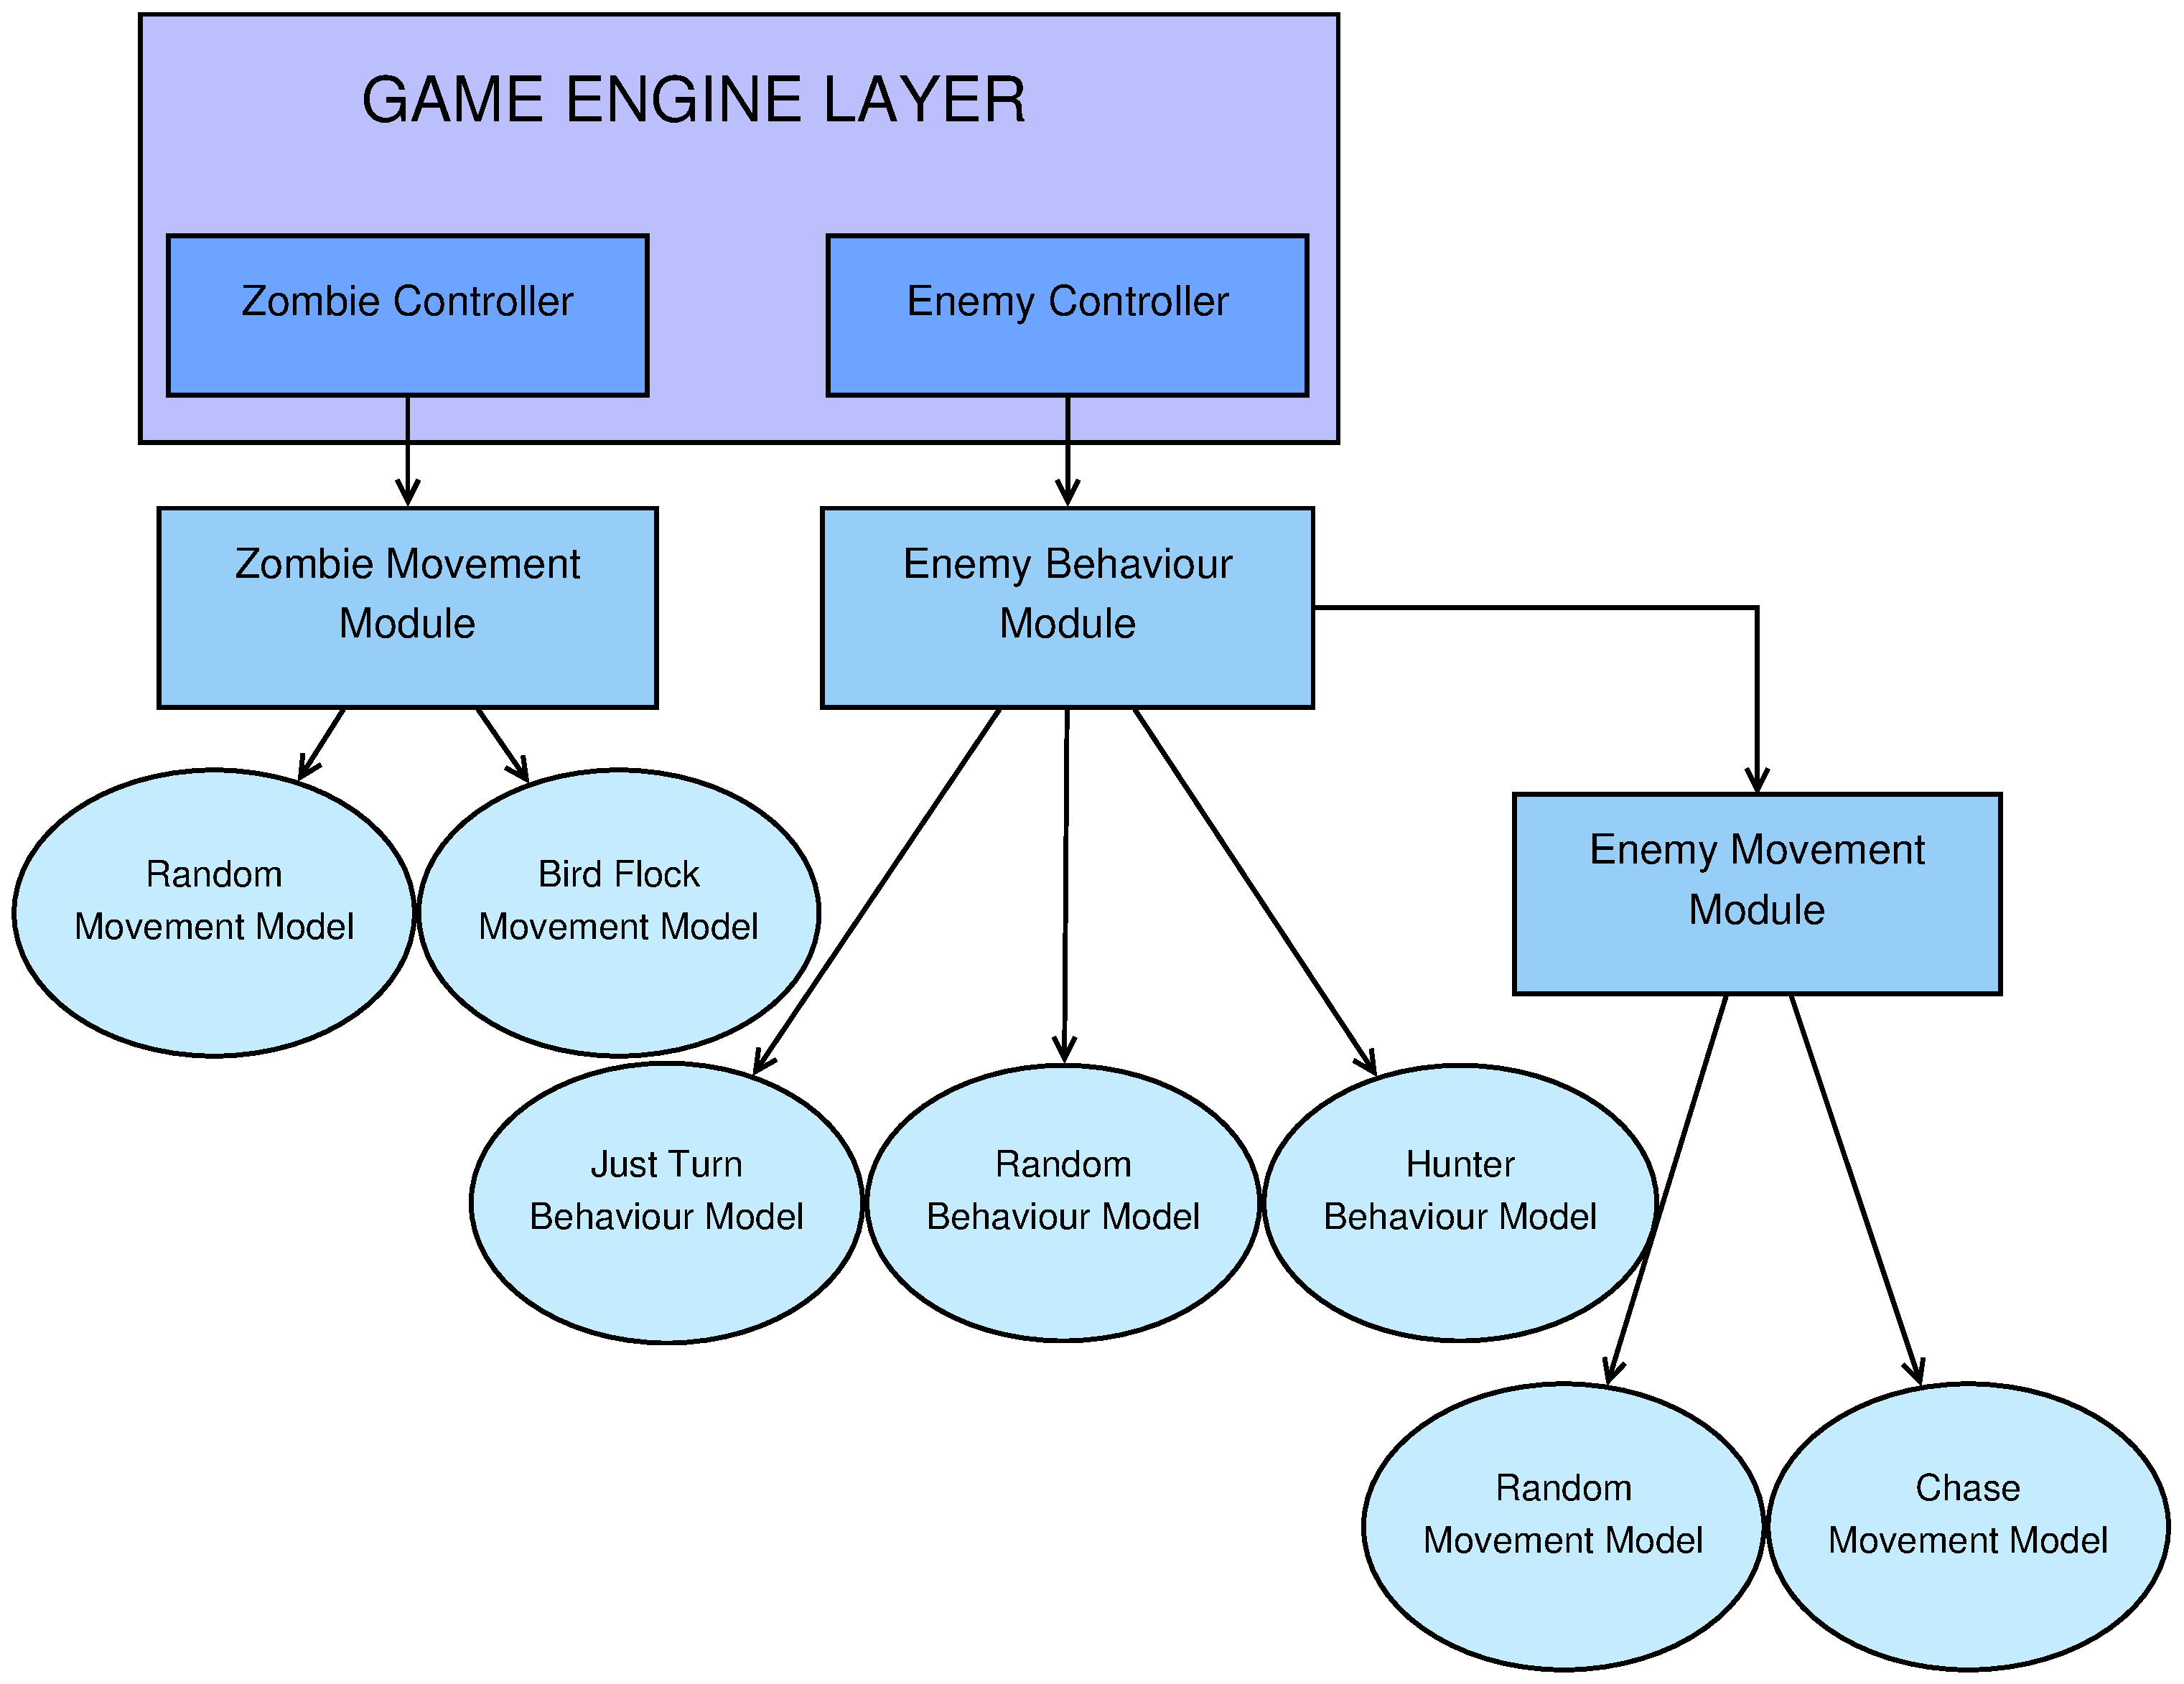
\includegraphics[scale=0.21]{modulos.eps}
	    \end{frame}

	\section{Conclusions}

	  \begin{frame}{Developing costs}
	    According to our experience and using the repository statistics as an approximate measure, we can estimate the cost of the developing in about: \newline

	    \begin{center}
	     \begin{tabular}{cc}

		\hline
		\textbf{Concept}	& \textbf{Hours} \\
		\hline
		Ogre formation		& 20 \\
		System Design		& 12 \\
		Programming		& 70 \\
		Artwork			& 12 \\
		Documentation		& 24 \\
		\hline
	  \newline    
	     \end{tabular}
	    \end{center}
	  
	  To summarize, we have invest in the project a total of \textbf{138 hours}. As a curiosity the code contains about \textbf{4242 lines}.
	  \end{frame}

	\begin{frame}{The End...}
	    \includegraphics[scale=0.5]{questions.png}
	\end{frame}


\end{document}
